% ------------------------------------------------------------------------
% ------------------------------------------------------------------------
% ------------------------------------------------------------------------
%                              Introducción
% ------------------------------------------------------------------------
% ------------------------------------------------------------------------
% ------------------------------------------------------------------------

\nnchapter{INTRODUCCIÓN}
% ------------------------------------------------------------------------
% ------------------------------------------------------------------------
Los cerámicos con estructura cristalográfica tipo perovskita han sido parte fundamental de la ciencia y tecnología gracias a la variedad de propiedades físicas que pueden llegar a adquirir \cite{Howard2005StructuresApproach,Sarmiento-Perez2015PredictionPerovskites}. Los acoplamientos y alteraciones que se han realizado desde el descubrimiento del mineral titanato de calcio ($CaTiO_{3}$), también conocido como perovskita, han sido esenciales para encontrar nuevas propiedades magnéticas y eléctricas, consiguiendo materiales aislantes\cite{Tokura1997Metal-insulatorOxide}, conductores\cite{Chen2017Atomic-ScaleStructures}, semiconductores\cite{Garcia-Esparza2019FullFuels} y superconductores\cite{Maeno1994SuperconductivityCopper}, hasta materiales multiferroicos\cite{Cruz2014PiezoelectricThickness}, magnetoeléctricos\cite{Fiebig2005RevivalEffect} y materiales multiferróicos magnetoeléctricos\cite{Hill2000WhyFerroelectrics}. La versatilidad de la perovskita cúbica $ABX_{3}$ permite distintas posibilidades de agrupación, consiguiendo sistemas laminares, los cuales son formados por capas que crecen en una dirección específica, como la perovskita doble, Dion-Jacobson, Ruddlesden-Popper y Aurivillus \cite{Benedek2015Undestanding}.

\begin{figure}[h!]
    \centering
    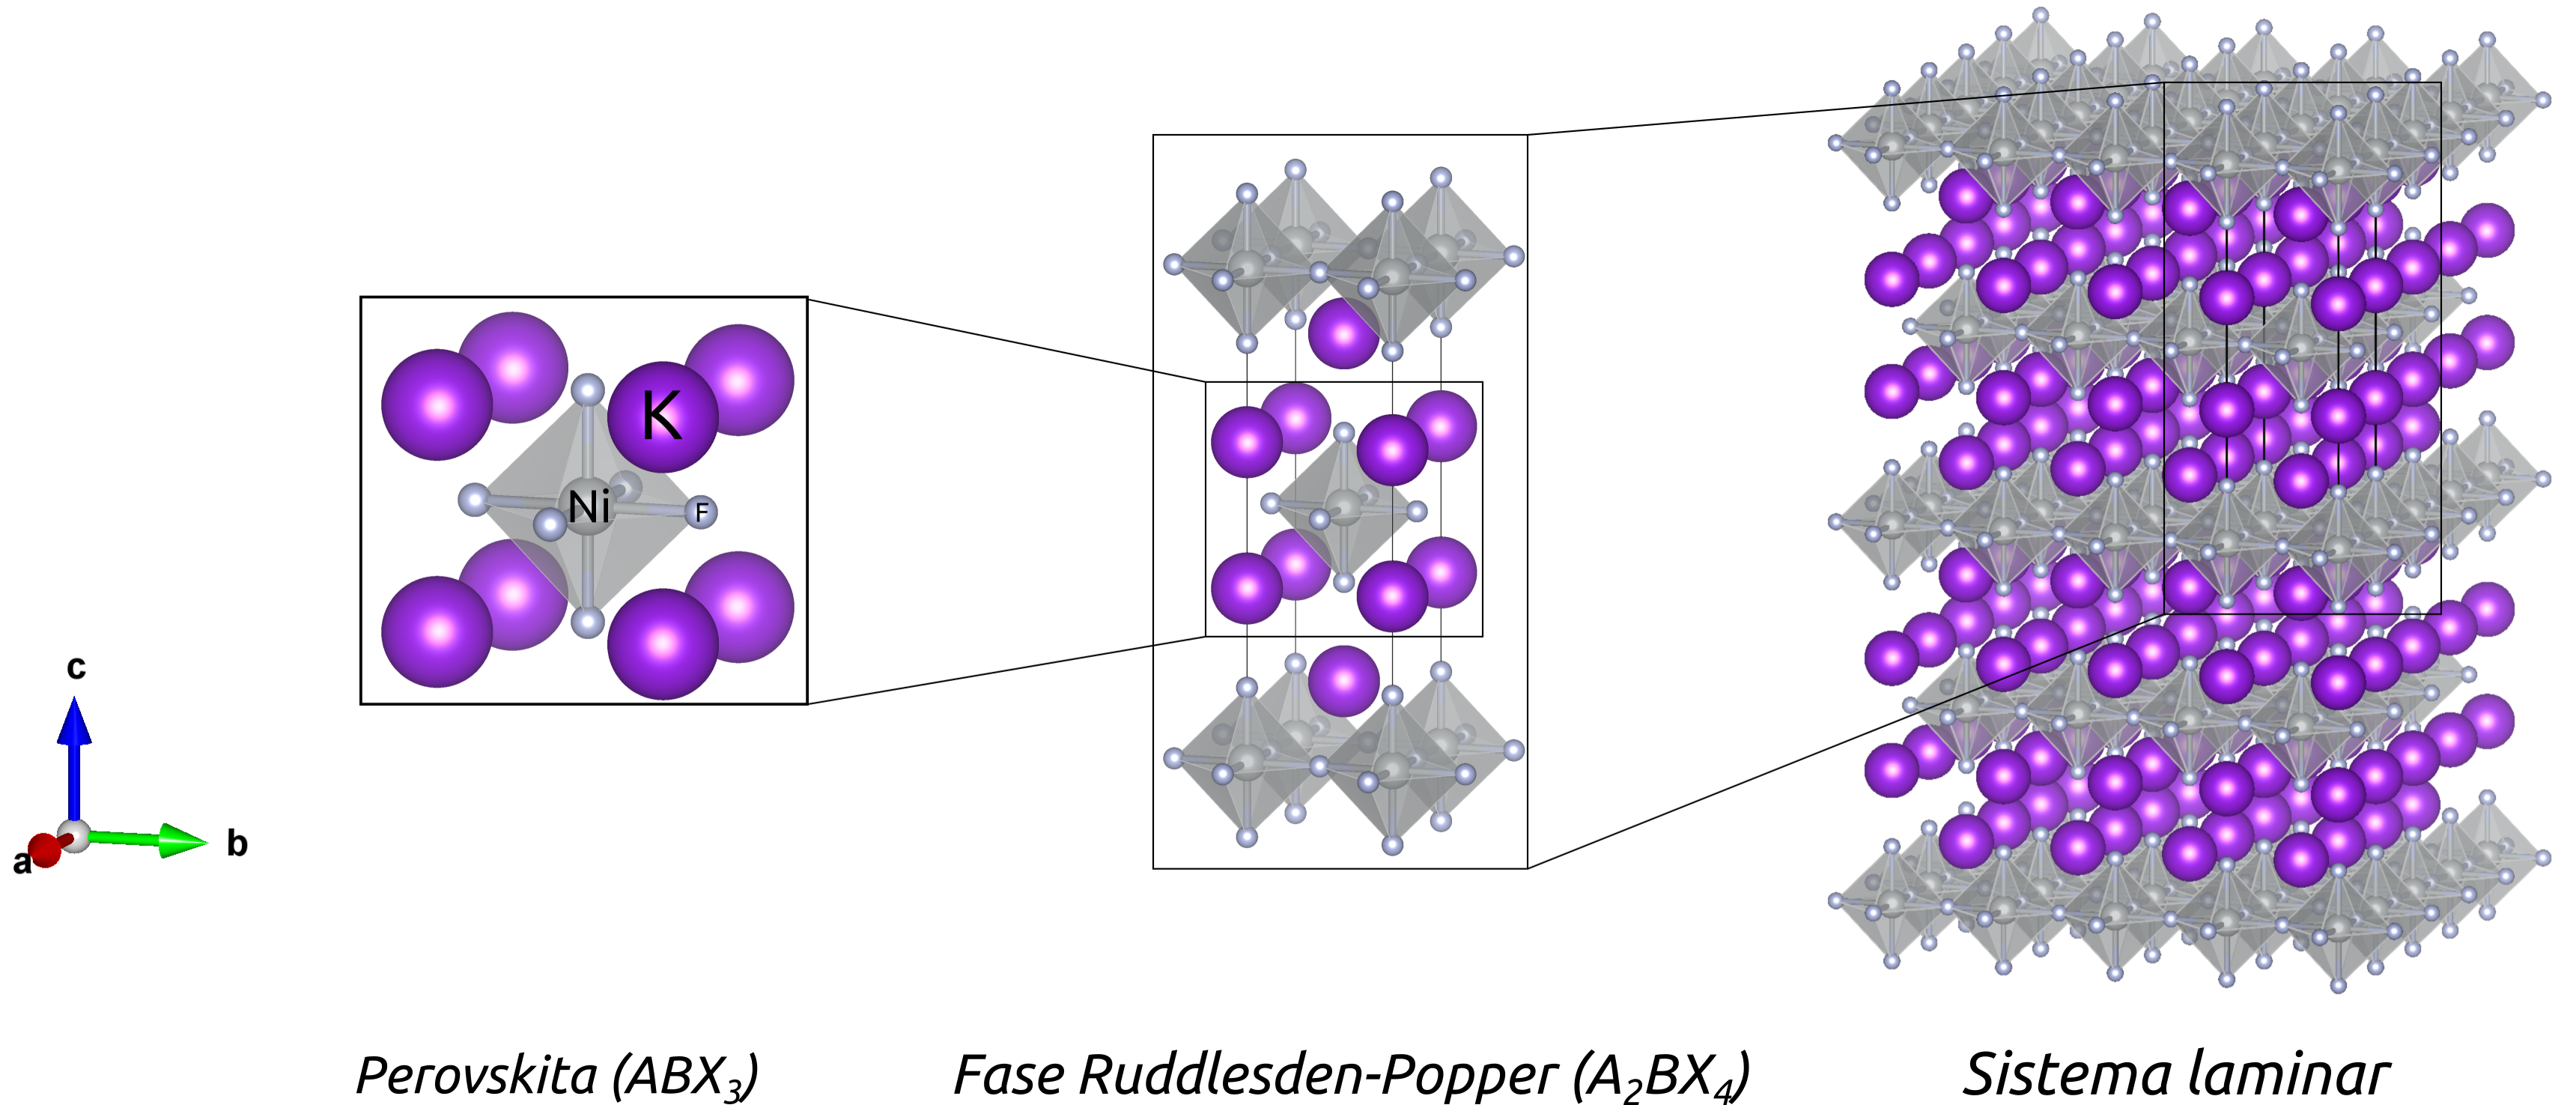
\includegraphics[width=13.0cm,keepaspectratio=true]{Figs/material1.png}
    \caption{Estructura $K_{2}NiF_{4}$ de la familia de estructuras tipo Ruddlesden-Popper \cite{NRuddl1957NewType}.}
    \label{fig:k2nif4}
\end{figure}

La figura \ref{fig:k2nif4} muestra un sistema laminar de perovskitas distribuidas por capas dislocadas formando la familia de estructuras Ruddlesden-Popper, la cual se descubrió en el material $K_{2}NiF_{4}$. Algunos ejemplos son: $Sr_{2}TiO_{4}$, $Ca_{2}MnO_{4}$ y $Sr_{2}LaAlO_{4}$ \cite{NRuddl1957NewType}. La familia \textsc{rp} se distingue por su formula química $A_{n+1}B_{n}X_{3n+1}$, donde $n$ indica la fase de la estructura dentro de la familia \textsc{rp} \cite{Fuertes2012ChemistryPerovskites}. En el presente trabajo, la fase considerada es $n=1$ que lleva a la fórmula química $A_{2}BX_{4}$, donde los átomos $A$ y $B$ son cationes y los átomos $X$ son aniones \cite{Clarke2002}. Esta fase \textsc{rp} es formada si los sitios cristalográficos $A$ son ocupados por cationes más grandes, indicando que deben tener valencias de $1+$ o $2+$ \cite{Beznosikov2000}, como es el caso del estroncio ($Sr^{2+}$) al disponerlo en la celda unitaria. De esta manera, la fase \textsc{rp} toma la forma $Sr_{2}BX_{4}$. Este proyecto se enfoca en dos materiales con diferente metal de transición: tántalo y niobio $(Ta,Nb)$, ocupando el sitio cristalográfico $B$, ya que estos cationes al combinarlos con nitrógeno pasarán de una oxidación $4+$ a una oxidación $5+$, lo cual hace a la estructura mas estable, como ocurre en el caso de la perovskita $SrNbO_{2}N$ \cite{Tobias2004}. El átomo de oxigeno ocupa el sitio $X$ dando la forma a la estructura $Sr_{2}(Ta,Nb)O_{4}$. El enfoque que se le da a esta estructura consiste en la variación de la concentración de oxígeno, sustituyendo estos aniones por átomos nitrógeno, dando lugar a la estructura oxinitrada $Sr_{2}(Ta,Nb)O_{4-x}N_{x}$, para encontrar nuevas estructuras cristalográficas que exhiben propiedades como fotocatálisis para división de agua y comportamiento  ferroeléctricos debido a la dependencia del ordenamiento aniónico
\cite{Bouri2018,Morgan1986,Page2007LocalTheory}.

La perovskita tipo Ruddlesden-Popper ha atraído la atención como un posible nuevo material ferroeléctrico debido al orden aniónico en la estructura cristalina \cite{Gou2020Photocatalysis}. Se han reportado oxinitruros de metales de transición sensibles al orden de óxido-nitruro, alterando las propiedades ópticas, foto-catalíticas, dieléctricas y magnetorresistivas, además de ser más estables en el aire y la humedad que los nitruros puros\cite{Yang2011}. Los oxinitruros a menudo exhiben colores brillantes y una resistividad significativamente menor en comparación con los óxidos puros de metales de transición com $Ti^{5+}$, $Nb^{5+}$ o $Ta^{5+}$ \cite{Ebbinghaus2004}. Una forma de obtener oxinitruros a partir de oxidos puros es realizar substituciones atómicas de los sitios cristalográficas para determinar la disposición de los átomos sustituidos en la estructura, a través del código \textit{Site Ocupanccy Disorder} (\textsc{sod}) \cite{Grau-Crespo2007}.

El presente trabajo de grado expone una investigación teórica mediante la teoría funcional de la densidad (\textsc{dft}), basada como su nombre lo indica, es una funcional de la densidad electrónica de todo el sistema. Las funciones de onda se pueden expresar en términos de esta densidad electrónica y resolver la ecuación de Schrödinger simplemente definiendo el funcional de la densidad con solo tres variables espaciales en lugar de $3N$ variables.\cite{ACGarcia2016phd}. Esta investigación teórica permitirá caracterizar el material mediante el análisis de sus propiedades, de su estructura electrónica y estructura fonónica.

El capítulo uno de esta tesis se abordan conceptos fundamentales de perovskitas tipo \textsc{rp}, materiales oxinitrados y sus propiedades. En el componente teórico se incluye la teoría funcional de la densidad (\textsc{dft}), el parámetro \textsc{u} construido en \textsc{dft+u}, además del modelo de aproximación armónica y la corrección no analítica \cite{Wang_2010-nac} implementado en el código \textsc{phonopy} \cite{Togo2015phonopy}, para calcular la dispersión de fonones. En el capitulo dos se realiza un análisis de las sustituciones aniónicas y la relajación estructural de las configuraciones \textsc{rp} encontradas, junto con su caracterización como los parámetros de red, el volumen de la celda y el grupo espacial. Posteriormente en el capítulo tres se discute la estructura electrónica de las configuraciones mas estables energéticamente, además de su posible aplicación en fotocatálisis para división de agua. Luego se analiza la estructura fonónica de las configuraciones mas favorables con ordenamiento aniónico \emph{trans} y \emph{cis} para encontrar fases polares que lleven a una posible ferroelectricidad. Finalmente se presentan las conclusiones, recomendaciones y posibles trabajos futuros conseguidos en el desarrollo de la investigación.



% ------------------------------------------------------------------------
% ------------------------------------------------------------------------